\begin{figure*}[htbp]
    \centering
    \begin{tabular}{m{75mm} m{75mm} m{20mm}}
        \begin{minipage}[b]{75mm}
            \centering
            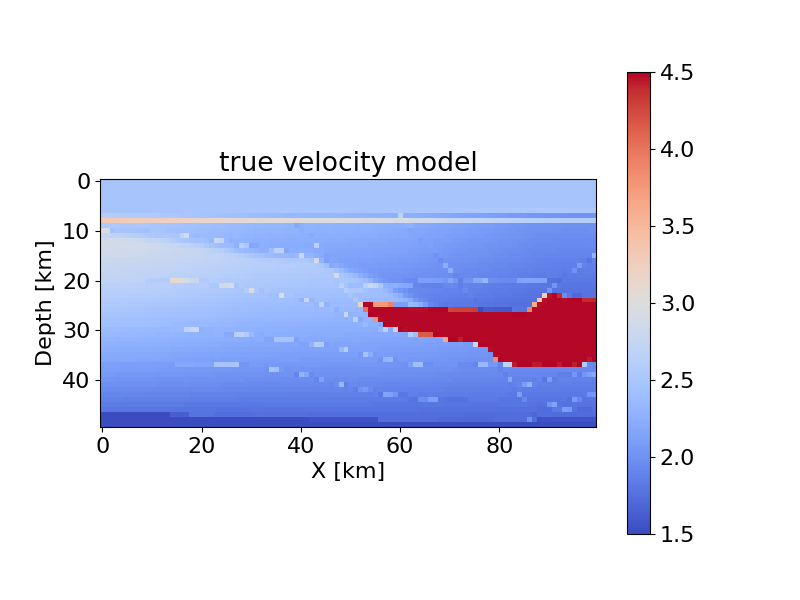
\includegraphics[width=75mm]{public/true}
            \vspace{-9mm}
            \caption*{\raisebox{2mm}{Background truth}}
        \end{minipage} &
        \begin{minipage}[b]{75mm}
            \centering
            
\includegraphics[width=75mm]{public/initial}
            \vspace{-9mm}
            \caption*{\raisebox{2mm}{Initial model}}
        \end{minipage} &
        \multirow[t]{3}{*}{\raisebox{-52.5mm}{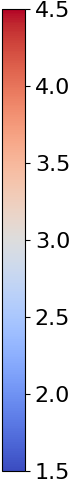
\includegraphics[height=75mm]{public/color-bar}}} \\

        \begin{minipage}[b]{75mm}
            \centering
            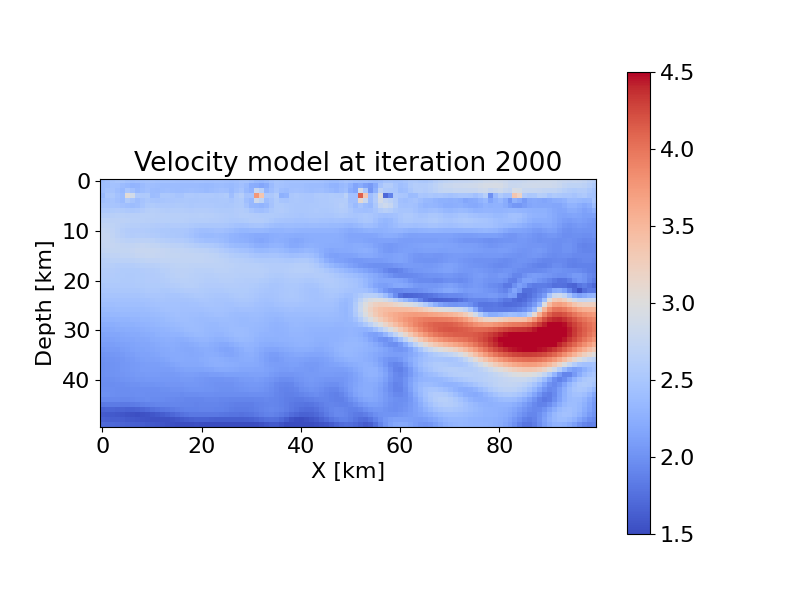
\includegraphics[width=75mm]{public/gradient}
            \vspace{-9mm}
            \caption*{\raisebox{2mm}{The Standard FWI Method}}
        \end{minipage} &
        \begin{minipage}[b]{75mm}
            \centering
            \vspace{-2mm}
            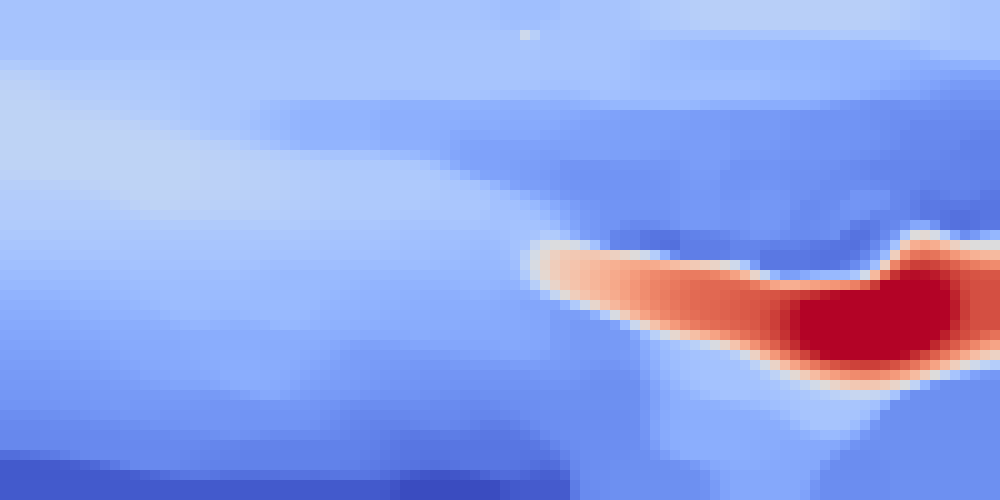
\includegraphics[width=75mm]{public/alpha_350}
            \vspace{-11mm}
            \caption*{The Proposed Method, $\alpha = 350$}
        \end{minipage} \\
    \end{tabular}
    \caption{Velocity models and their corresponding reconstructions.}
    \label{fig:velocity-models}
\end{figure*}

\subsection{Experimental Setup}\label{subsec:experimental-setup}

To demonstrate the effectiveness of the TV and box constrained FWI, we conducted FWI experiments where we compared with the standard FWI method\footnote{
    \begin{equation} \label{eq:FWIWithGradient} \FWIWithGradient, \end{equation} where $\gamma$ is the step size.
}\cite{FWI0}, using the SEG/EAGE Salt and Overthrust Models.

The velocity model consists of 51 $\times$ 101 grid points.
The ground truth velocity model is generated by zooming and cropping Fig.~\ref{fig:salt-model}.
The initial velocity model is generated by smoothing the ground truth velocity model with a Gaussian function with a standard deviation of 80.
The source waveform is a Ricker wavelet with a peak wavelet frequency of 10 Hz.
The number of waveform sources and receivers is 20 and 101, respectively, and they are placed on the surface at equal intervals.
The gradient $\nabla E$ is computed numerically using the Devito framework\cite{devito}.
The number of iterations is set to 5000.
In the standard FWI, the step size $\gamma$ is set to $1.0 \times 10^{-4}$.
In our algorithm, the step size $\gamma_1$ and $\gamma_2$ are set to $1.0 \times 10^{-4}$ and $1.0 \times 10^2$, respectively.
The lower and upper bounds of the velocity model $l$, $u$ are set to 1.5[km/s] and 4.5[km/s], respectively.
The experiments are conducted with several $\alpha$, that is, the upper bound of the $l_{1,2}$ norm.
%However, it should be noted that parameters such as $\alpha$, $a$, and $b$ were determined by referencing the ground truth data.
%In a practical application, this must be determined independently of this framework.


\subsection{Results and Discussion}\label{subsec:results-and-discussion}

\begin{figure}[htbp]
    \centering
    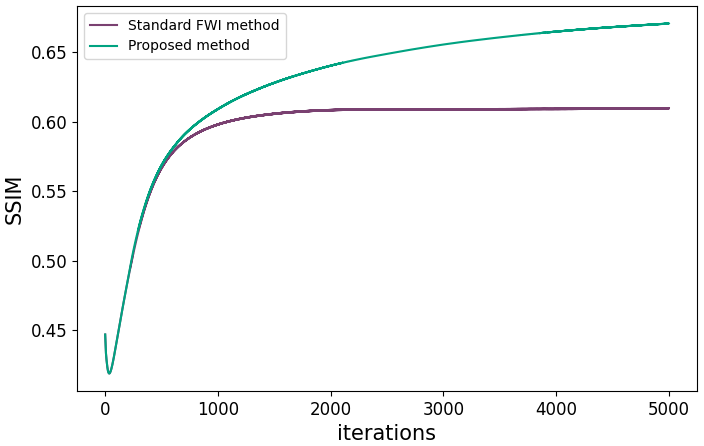
\includegraphics[width=\linewidth]{public/iters-ssim}
    \caption{SSIM against the number of iterations.}
    \label{fig:iters-ssim}
\end{figure}


\begin{figure*}[htbp]
    \centering
    \begin{tabular}{m{75mm} m{75mm} m{20mm}}
        \begin{minipage}[b]{75mm}
            \centering
            \vspace{-1mm}
            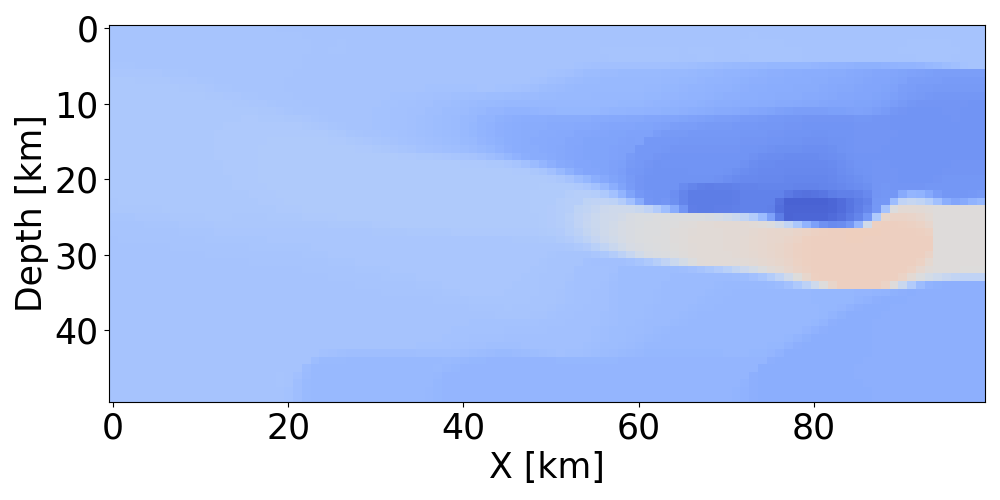
\includegraphics[width=75mm]{public/alpha_150}
            \vspace{-10mm}
            \caption*{The Proposed Method, $\alpha = 150$}
        \end{minipage} &
        \begin{minipage}[b]{75mm}
            \centering
            \vspace{-1mm}
            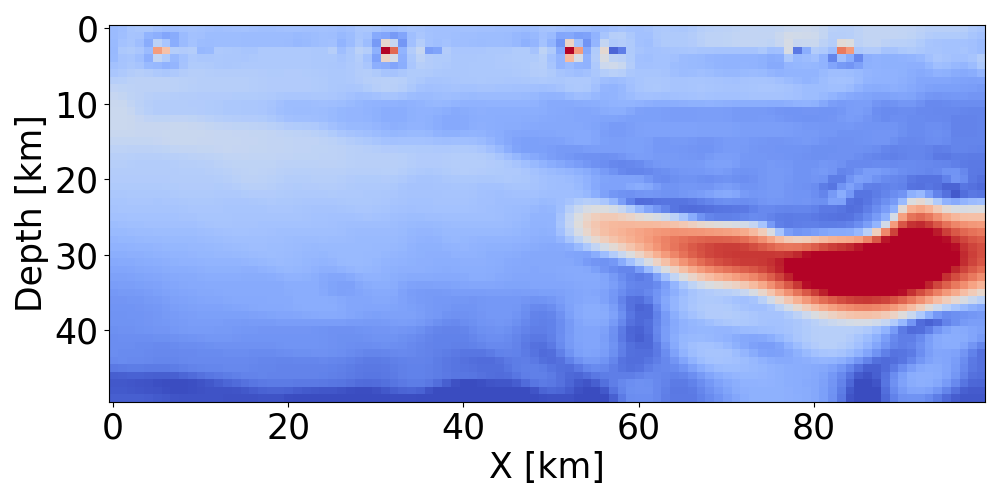
\includegraphics[width=75mm]{public/alpha_550}
            \vspace{-10mm}
            \caption*{The Proposed Method, $\alpha = 550$}
        \end{minipage} &
        \multirow[t]{3}{*}{\raisebox{-8.5mm}{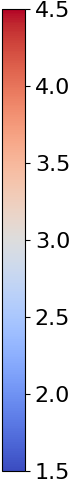
\includegraphics[height=29.5mm]{public/color-bar}}} \\
    \end{tabular}
    \caption{Reconstructed velocity models by proposed method with several $alpha$.}
    \label{fig:reconstructed-velocity-models-with-several-alpha}
\end{figure*}


Fig.~\ref{fig:velocity-models} shows the ground truth, the initial model, and the reconstructed velocity models using the standard FWI method and the proposed method with the best parameter of $\alpha = 350$.
The standard FWI method introduces wave-like artifacts and noise around the source positions, which negatively affects the accuracy of the reconstructed velocity model.
In contrast, The enhancements in the proposed method are particularly evident as it successfully eliminates these artifacts and noise, resulting in a more accurate velocity model reconstruction.
To quantify this further, we plot the Structural Similarity Index Measure (SSIM) against the number of iterations for both methods in Fig.~\ref{fig:iters-ssim}.
In this case, the proposed method consistently achieves higher SSIM values than the standard FWI method at every iteration, also indicating enhanced reconstruction accuracy.

\begin{figure}[htbp]
    \centering
    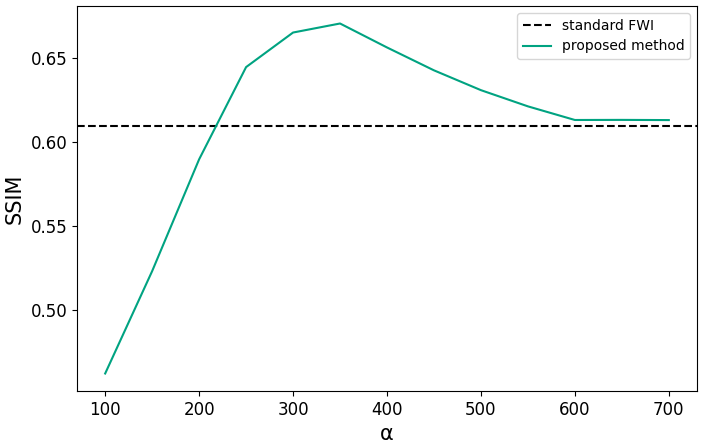
\includegraphics[width=\linewidth]{public/alpha-ssim}
    \caption{SSIM against the parameter of alpha.}
    \label{fig:alpha-ssim}
\end{figure}

To investigate the effect of the parameter $\alpha$, we show the reconstructed velocity models using the proposed method with multiple $\alpha$ in Fig.~\ref{fig:reconstructed-velocity-models-with-several-alpha}.
When $\alpha$ is as small as 150, the TV constraint is too strong, resulting in an excessively smooth model.
Conversely, when $\alpha$ is as large as 550, the TV constraint is almost meaningless, and the model is similar to that obtained by the standard FWI method.
For a more detailed analysis, we plot the SSIM at the last iterations against the parameter $\alpha$ in Fig.~\ref{fig:alpha-ssim}.
As mentioned earlier, the graph shows that when the value of $\alpha$ is small, the last SSIM decreases, and when the value of $\alpha$ is too large, the results become almost the same as the standard FWI method, but not worse, and when the value of $alpha$ is appropriate, high SSIM values can be achieved.
This demonstrates that the parameter $\alpha$ has a clear and predictable effect on the reconstructed velocity model, allowing for easy adjustment to achieve accurate results.
